	\chapter{Programmation impérative en C}
	Énormément de langage sont fondés sur la syntaxe du langage C.

	Il a été développé dans les années 1960 par Dennis Ritchie. 

	On trouvera toujours une partie description de l'organisation des données en mémoire\footnote{C'est un grand tableau découpé en cases mémoire.},
	nous aurons donc une déclaration de variables et un type de données.
	\begin{lstlisting}[caption=Syntaxe de déclaration de variable]
type nomVariable;		
	\end{lstlisting}
	\section{Description de l'organisation des données en mémoire}\label{types}
	Le C possède différents type de données: 
	\begin{description}
		\item[int] Entiers signés
		\item[unsigned int] Entiers non signés 
		\item[float] Nombre réel sur 32bits. 
		\item[double] Nombre réel sur 64bits.
		\item[char] Entier signé sur 8bits.
		\item[pointeur] type* ptr; La case mémoire contient une adresse.
	\end{description}
	\section{Code syntaxe}
	\subsection{Blocs}
\begin{lstlisting}[language=C, caption=Syntaxe d'un bloc]
bloc { // début du bloc
} //fin du bloc
\end{lstlisting}
	Toute variable est visible dans son bloc de déclaration et ses blocs imbriqués.

	Un bloc transforme une séquence en action.

	\subsection{Séquence}\label{sequence}
\begin{lstlisting}[language=C, caption=Syntaxe des actions]
action 1;
action 2;
action 3;
\end{lstlisting}
\subsection{Séléction}\label{selection}
\begin{lstlisting}[language=C, caption=Syntaxe d'une structure de contrôle]
if(conditon) {
	action 1;
} else {
	action 2;
}
\end{lstlisting}
Condition est une expression booléenne\footnote{Expression renvoyant vrai($\neq 0$) ou faux($=0$)}, si celle-ci est vrai, action 1 est executé, sinon action 2 est executé. 

\subsection{Répétition}\label{repetition}
\begin{lstlisting}[language=C, caption=Syntaxe de répétition]
while(condition) {
	action;
}
\end{lstlisting}
Condition est une expression booléenne, tant que la condition est vrai, les actions se répètent.

\subsection{Affectation}\label{affectation}
\begin{lstlisting}[language=C, caption=Syntaxe d'une affectation ]
variable = expression;
\end{lstlisting}
variable reçoit expression, si celle-ci n'est pas du même type que variable, un cast\footnote{ou conversion de type, consiste à convertir un type vers un autre. (int vers double par exemple)} peut-être effectué.
\newpage
\subsection{Opérateurs de base sur les types}
\begin{description}
	\item[\texttt{=}] Affectation
	\item[\texttt{+}, \texttt{-}, \texttt{/}, \texttt{*}] Opérateurs arithmétiques.
	\item[\texttt{\&\&}, \texttt{||}, \texttt{!}] Opérateurs logiques 
	\item[\texttt{==}, \texttt{!=}, \texttt{<}, \texttt{>}, \texttt{<=}, \texttt{>=}] Opérateurs booléens
	\item[\texttt{+$\,$+i}, \texttt{i+$\,$+}, \texttt{-$\,$-i}, \texttt{i-$\,$-}] Opérateur unaires d'incrémentation.
	\item[\texttt{\&}, \texttt{\^}, \texttt{|}, \texttt{<$\,$<}, \texttt{>$\,$>}] Opérateurs binaires
\end{description}
\subsection{Opérateurs d'entrées / sorties}
\paragraph{Ecriture}~\\
\begin{lstlisting}[language=C, caption=Syntaxe de l'appel de printf]
printf('format', var1, var2);
\end{lstlisting}
La chaine format peut contenir une chaine de caractères, avec des caractères spéciaux : 
\begin{description}
	\item[\texttt{'\%d'}] Entier sous forme décimale
	\item[\texttt{'\%ox'}] Entier sous forme hexadécimale
	\item[\texttt{'\%f'}] Flottant 
	\item[\texttt{'\%c'}] Caractère 
	\item[\texttt{'\%s'}] Chaine de caractères 
	\item[\texttt{'\\n'}] Vide le buffer et fait un retour chariot 
	\item[\texttt{'\\t'}] Tabulation 
	\item[\texttt{'\\r'}] Revient en début de ligne.
	\item['\ldots'] RTFM	
\end{description}
Les différents formats doivent être dans l'ordre des variables passés en paramètres.
\paragraph{Lecture}~\newline
\begin{lstlisting}[language=C, caption=Syntaxe de l'appel de scanf]
scanf('format', &var1); // & représente l'adresse de la variable dans laquelle écrire.
\end{lstlisting}
\attention{L'utilisation de cette fonction est risquée. En effet, un utilisateur malveillant peut écrire à des cases mémoires où il n'est pas autorisé.}

\subsection{Tableaux}
Un tableau est une collection d'éléments de même type.
\begin{lstlisting}[language=C, caption=Syntaxe de déclaration d'un tableau]
// avec tableau le nom de la variable et N la taille du tableau. 
type tableau[N], i; 
i = tableau[P]; //i recoit la valeur de la case P du tableau
\end{lstlisting}
\attention{Un tableau commence toujours à 0 et finit à N-1, ainsi, il faut faire très attention au dépassement de la taille d'un tableau.}
\subsection{Les sous-programmes}
Un sous-programme est un sous-ensemble du programme dans sa hiérarchie fonctionnelle. En C, il correspond toujours à une fonction ou une procédure.
\begin{lstlisting}[language=C, caption=Syntaxe d'un sous programme]
typeRetour nomFonction (typeArg1 nomArg1, typeArg2 nomArg2) {
	/*
     *	code
	 */
	 [return (valeur)];
}
\end{lstlisting}
\texttt{typeRetour} peut posséder comme valeur les même types qu'une variable, voir \ref{types} page \pageref{types}. Celui-ci peut également être \texttt{void}, 
cela signifie que que la fonction ne renvoie rien, c'est donc une procédure.
\section{Structure d'une programme en C}
\begin{tabular}{p{8cm}|p{8cm}}
	\textbf{Interface} & \textbf{Implantation}\\
	\begin{minipage}{0.8\textwidth}
		\begin{itemize}
			\item Déclaration des fonctions (prototype)
			\item Constantes, types
			\item Comment utiliser le programme\\~~~~ $\Rightarrow$ \'Ecrire dans un fichier .h (header)
			\item Préprocesseur (define, macros, \ldots)
		\end{itemize}
	\end{minipage}&
	\begin{minipage}{0.8\textwidth}
		\begin{itemize}
			\item Définitions des fonctions: le code\\~~~~ $\Rightarrow$ \'Ecrire dans un fichier .c
		\end{itemize}
	\end{minipage}
\end{tabular}
Un programme en C ne possède qu'une seul point d'entrée : une instruction est exécuté, c'est la fonction \texttt{main}.
\begin{lstlisting}[language=C, caption=Point d'entrée du programme: le main]
int main (int argc, char **argv); 
//le programme renvoie un entier. C'est le profil d'une fonction.
\end{lstlisting}

\section{La compilation}
\begin{figure}[H]
	\centering
	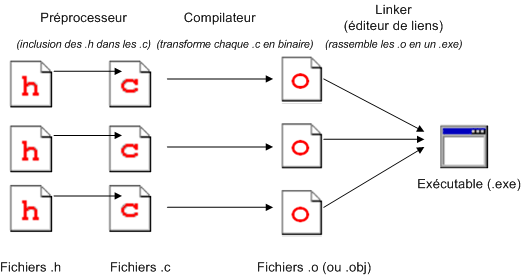
\includegraphics[width=13.5cm]{compilation.png}
	\caption{La compilation}
\end{figure}
\subsection{\'Etape 1 : Le préprocesseur}
Le pré processeur sont les instructions situés en dehors d'un programme, ceux-ci sont préfixé par un dièse (\#).
\begin{description}
	\item[Entrée] fichier.c
	\item[Sortie] fichier obtenu une fois les modifications effectués.
\end{description}~
\begin{lstlisting}[language=C, caption=Exemple d'instructions pré-processeurs]
#include // remplace par le continu du fichier inclus
#define Arg1 Arg2 // remplace syntaxique de Arg1 par Arg2
\end{lstlisting}
\subsection{Etape 2 : La compilation}
\begin{description}
	\item[Entrée] fichier.c, fichier.h
	\item[Sortie] fichier.o 
\end{description}
\begin{lstlisting}[language=bash]
gcc -c fic1.c fic2.c fic3.c # Créé les fichiers .c
gcc *.o nomExe #Créer l'executable.
\end{lstlisting}
\remarque{La compilation sera étudiée en détails lors des cours de L3 et M1}
\subsection{\'Etape 3 : L'édition de liens}
Rassemble tous les fichiers binaires .o en un seul executable.
